\documentclass[
    11pt, % Set the default font size, options include: 8pt, 9pt, 10pt, 11pt, 12pt, 14pt, 17pt, 20pt
    aspectratio=169, % Set the aspect ratio to a 16:9 ratio which matches the aspect ratio of 1080p and 4K screens and projectors
]{beamer}

% This template is inspired by the VT Presentation Template, as well as the THU Beamer Theme. Many thanks!

\graphicspath{{images/}{./}} % Specifies where to look for included images (trailing slash required)
\usepackage{booktabs} % Allows the use of \toprule, \midrule and \bottomrule for better rules in tables
\usepackage{calligra} % Font for wordart
% \usepackage{appendixnumberbeamer} % If you want a separate slide counter for your appendix
\usepackage{fnpct} % Eliminate the unwanted space before the footnote mark
\usepackage{listings} % For code display

%---------------------------------------------------------
%	FOOTNOTES & CITATIONS BASIC SETUP
%---------------------------------------------------------
% Check FOOTNOTES & CITATIONS ADVANCED SETUP for solutions for intra- and inter-frame citations
% The workarounds in ADVANCED SETUP require the style to be "numeric"
% If you're good without ADVANCED SETUP, comment out the ADVANCED SETUP section, and pick whatever style you like
% \usepackage[style=authoryear, backend=bibtex]{biblatex}
\usepackage[style=numeric, sorting=none, backend=biber]{biblatex}
\addbibresource{bib.bib}
\setbeamerfont{footnote}{size=\tiny}
% The lines below set the citation style to "number, title, year". The ADVANCED SETUP will overwrite this style
\usepackage{xpatch}
\xapptobibmacro{cite}{\setunit{\nametitledelim} \printfield{title} \setunit{\nametitledelim} \printfield{year}}

%---------------------------------------------------------
%	FOOTNOTES & CITATIONS ADVANCED SETUP
%---------------------------------------------------------
% Manage faulty intra- and inter-frame footnotes and citations. References:
%     https://tex.stackexchange.com/a/520777
%     https://topanswers.xyz/tex?q=453

% You might want to use \firstcite and \secondcite instead of \footnote in your document
% Mark the first citation with \firstcite and the rest with \secondcite

% \renewcommand{\thefootnote}{\arabic{footnote}} % Switch to footnote with numbers
% \renewcommand{\thefootnote}{\alph{footnote}} % Switch to footnote with letters

\DeclareCiteCommand{\firstcite}
{\usebibmacro{prenote}}
{%
    \footnotemark[\thefield{labelnumber}]% mark corresponding to the number entry
    \footnotetext[\thefield{labelnumber}]{% footnote text corresponding to the number entry
        \printnames{labelname}% name
        \setunit{\printdelim{nametitledelim}}% separator
        % \setunit{\addperiod\space}% another way to add separator
        \printfield[citetitle]{labeltitle}% title
        \setunit{\printdelim{nametitledelim}}% separator
        \printfield{year}% year
        \newunit{\adddot}% ending dot
    }%
}
{\multicitedelim}
{\usebibmacro{postnote}}

\DeclareCiteCommand{\secondcite}
{\usebibmacro{prenote}}
{%
    \footnotemark[\thefield{labelnumber}]% mark corresponding to the number entry
}
{\multicitedelim}
{\usebibmacro{postnote}}

%---------------------------------------------------------
%	SELECT THEME & COLORS
%---------------------------------------------------------
\usetheme{Madrid} % You can use other themes too, but this changes many things. I've found Madrid to be the best for this color scheme

% fg = foreground color
% bg = background color

% Many colors are linked to multiple attributes, change with caution!
\definecolor{smuBlue}{RGB}{21, 28, 85}
% \definecolor{smuGold}{RGB}{138, 112, 76}
\definecolor{scisGold}{RGB}{198, 146, 0}

\setbeamercolor*{structure}{bg=smuBlue, fg=smuBlue}
% Title block and bottom right box color
\setbeamercolor*{palette primary}{use=structure, fg=white,bg=smuBlue} % Bottom left box and bar between title & top bubbles
\setbeamercolor*{palette secondary}{use=structure, fg=smuBlue, bg=white}
% Probably not used
\setbeamercolor*{palette tertiary}{use=structure, fg=white, bg=smuBlue} 

% Title of each slide
\setbeamercolor{frametitle}{bg=smuBlue, fg=white}
\setbeamercolor*{titlelike}{parent=palette primary}

%%% Headline and Central Footer %%%
% You can change the theme back and forth for each frame
% Theme I - white head, white foot
    % \setbeamercolor{section in head/foot}{fg=scisGold, bg=white}
    % \setbeamercolor{headline}{fg=scisGold, bg=white}
% Theme II - gold head, gold foot (as shown in the title frame)
    \setbeamercolor{section in head/foot}{fg=white, bg=scisGold}
    \setbeamercolor{headline}{fg=white, bg=scisGold}
% Theme III - white head, gold foot (as shown in the rest of the frames)
    % \setbeamercolor{section in head/foot}{fg=scisGold, bg=white}
    % \setbeamercolor{title in head/foot}{fg=white, bg=scisGold}
    % \setbeamercolor{headline}{fg=scisGold, bg=white}

%%% Specific Colors %%%
\setbeamercolor{item projected}{bg=scisGold}
\setbeamertemplate{enumerate items}{bg=scisGold}

\setbeamercolor{itemize item}{fg=scisGold}
\setbeamercolor{itemize subitem}{fg=scisGold}

\setbeamercolor{button}{bg=scisGold}

%%% Edits ONLY the TOC slide %%%
\setbeamercolor{section in toc}{fg=black}
\setbeamercolor{subsection in toc}{fg=black}

%%% Block Colors %%%
% Standard block
    \setbeamercolor{block title}{bg=scisGold, fg=white}
    \setbeamercolor{block body}{bg=scisGold!20}
% Alerted block
    \setbeamercolor{block title alerted}{bg=orange, fg=white}
    \setbeamercolor{block body alerted}{bg=orange!10}
% Example block
    \setbeamercolor{block title example}{bg=smuBlue, fg=white}
    \setbeamercolor{block body example}{bg=smuBlue!10}

%---------------------------------------------------------
%	SELECT THE FONT THEME & FONTS
%---------------------------------------------------------
\usefonttheme{default} % Typeset using the default sans serif font
\usepackage{palatino} % Use the Palatino font for serif text
\usepackage[default]{opensans} % Use the Open Sans font for sans serif text
\useinnertheme{circles}

%---------------------------------------------------------
%	SELECT THE OUTER THEME
%---------------------------------------------------------
% Outer themes change the overall layout of slides, such as header and footer lines, sidebars and slide titles. Uncomment each theme in turns to see what changes it makes to your presentation.

% \useoutertheme{default}
\useoutertheme{miniframes}
% \useoutertheme{infolines}
% \useoutertheme{smoothbars}
% \useoutertheme{sidebar}
% \useoutertheme{split}
% \useoutertheme{shadow}
% \useoutertheme{tree}
% \useoutertheme{smoothtree}

%---------------------------------------------------------
%	PRESENTATION INFORMATION
%---------------------------------------------------------
\title[SMU Beamer Template]{SMU Presentation Template}
% Click the middle footer can switch between the first and last numbered frame
\subtitle{Subtitle}
\author[For Internal Use]{Author: Felix Nie}

\institute[]{School of Computing and Information Systems \\ \smallskip \textit{email@smu.edu.sg}}
\date[Spring 2023]
% \date[\today]

% School logo
% You can enable and disable logo display for each frame
\logo{
\includegraphics[width=2.5cm]{logo.eps}}

%---------------------------------------------------------
%	CODE DISPLAY
%---------------------------------------------------------
\lstset{
    basicstyle=\ttfamily\small,
    keywordstyle=\bfseries\color{blue},
    emphstyle=\ttfamily\color{red},   
    stringstyle=\color{green},
    numbers=left,
    numberstyle=\small\color{gray},
    rulesepcolor=\color{red!20!green!20!blue!20},
    frame=shadowbox,
    xleftmargin=1cm,
    xrightmargin=1cm,
}

%---------------------------------------------------------
%	EXTRA SETTINGS
%---------------------------------------------------------

% Clear warnings related to \translate
%     https://github.com/josephwright/beamer/issues/449
\pdfstringdefDisableCommands{
    \def\translate#1{#1}
}

% Adjust header height
\setbeamertemplate{headline}{
    \nointerlineskip
    \begin{beamercolorbox}[wd=\paperwidth,ht=7.0ex]{headline}
        \insertnavigation{\paperwidth}\vspace*{2.0ex}
    \end{beamercolorbox}
}

% Disable navigation symbols
\setbeamertemplate{navigation symbols}{}

%---------------------------------------------------------
%   DOCUMENT BEGINS
%---------------------------------------------------------
\begin{document}

%---------------------------------------------------------
%	TITLE SLIDE
%---------------------------------------------------------
\section{}

% Set background
\usebackgroundtemplate{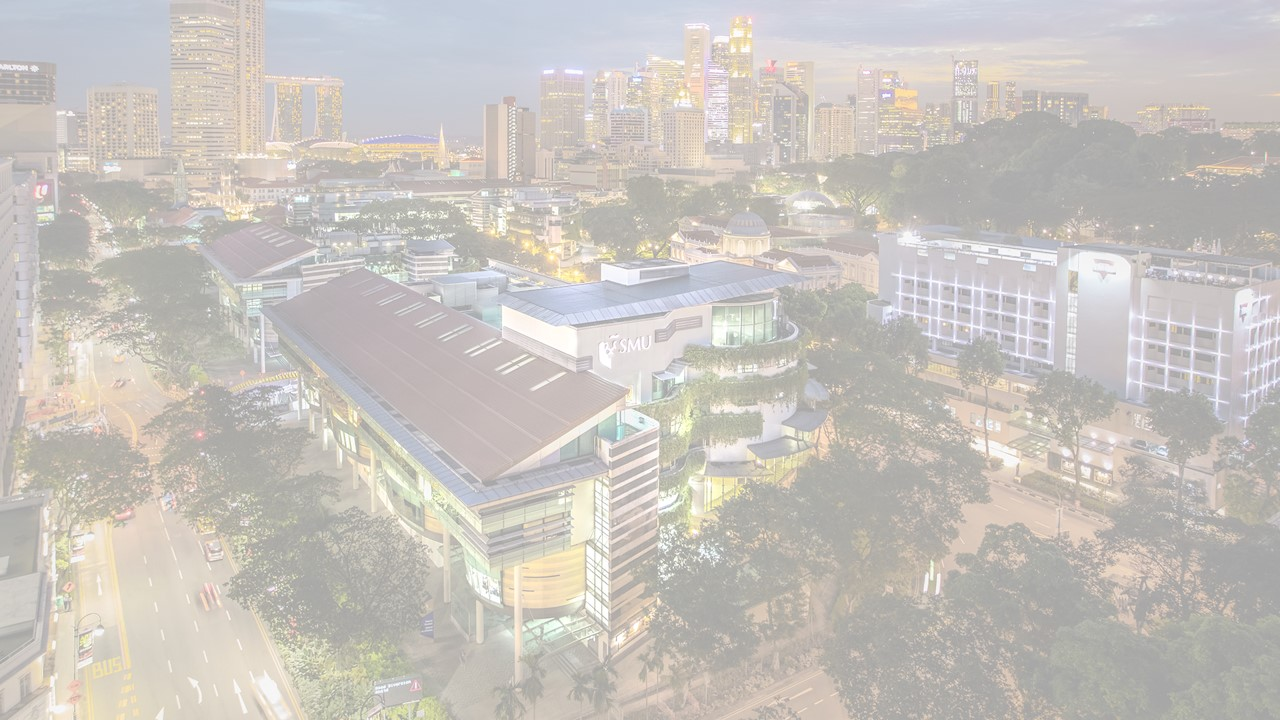
\includegraphics[width=\paperwidth]{background-1080p-washout.jpg}}
% Disable logo
\logo{}

\begin{frame}
	\titlepage % Output the title slide, automatically created using the text entered in the PRESENTATION INFORMATION block above
\end{frame}

% Clear background
\usebackgroundtemplate{}
% Enable logo
\logo{
\includegraphics[width=2.5cm]{logo.eps}}

% Switch to Theme III
\setbeamercolor{section in head/foot}{fg=scisGold, bg=white}
\setbeamercolor{title in head/foot}{fg=white, bg=scisGold}
\setbeamercolor{headline}{fg=scisGold, bg=white}

%---------------------------------------------------------
%	TABLE OF CONTENTS SLIDE
%---------------------------------------------------------
% References sections and subsections, specified with the standard \section and \subsection commands. If you want to display all sections and subsections on one slide, just use \tableofcontents. If you want to just display each section one at a time (in subsequent slides) use \tableofcontents[pausesections].

\begin{frame}
	\frametitle{Table of Contents} % Slide title, remove this command for no title
	
	\tableofcontents % Output the table of contents (all sections on one slide)
	%\tableofcontents[pausesections] % Output the table of contents (break sections up across separate slides)
\end{frame}
%---------------------------------------------------------
%	PRESENTATION BODY SLIDES
%---------------------------------------------------------
\section{Motivation} % Note all sections and subsections are automatically placed in your table of contents

%------------------------------------------------
\begin{frame}
    \frametitle{Title}
    \begin{center}
        \textbf{To use this template, just edit and add slides!} \newline
    \end{center}

    There are 3 color themes prepared for you under \textbf{Headline and Central Footer} section. \newline

    Check the color design of your school when customizing the theme: \newline

    \begin{center}
        \href{https://www.smu.edu.sg/about/university-brand-identity}{https://www.smu.edu.sg/about/university-brand-identity} \newline
    \end{center}

    The remainder of these slides serves as an example of the features you can use: footnotes, citations, columns, mini pages, bullets, links, code, maths, etc.

    \begin{center}
        {\Huge\calligra Enjoy!}
    \end{center}
\end{frame}

%------------------------------------------------
\begin{frame}
    \frametitle{Intra-frame Footnotes and Citations I}
    
    Citation in Beamer works slightly differently from conventional cites as Beamer rewrites its footnote and citation functions. 
    A common issue is the duplication of footnotes in a frame when using \texttt{footcite}. \newline

    This paper \footcite{Harshman1970}, that paper \footcite{Hitchcock1927}, and another paper \footcite{Carroll1970}. \newline

    And this paper \footcite{Harshman1970}, that paper \footcite{Hitchcock1927}, and another paper \footcite{Carroll1970} again. 
\end{frame}

%------------------------------------------------
\begin{frame}
    \frametitle{Inter-frame Footnotes and Citations I}

    Another issue with \texttt{footcite} is the unwanted continuation of the footnote index. \newline

    This paper \footcite{Harshman1970}, that paper \footcite{Hitchcock1927}, and another paper \footcite{Carroll1970}. \newline

    And this paper \footcite{Harshman1970}, that paper \footcite{Hitchcock1927}, and another paper \footcite{Carroll1970} again. \newline

\end{frame}

%------------------------------------------------
\begin{frame}
    \frametitle{Intra-frame Footnotes and Citations II}
    
    This template provides a workaround for these issues. 
    Let's use the customized command \texttt{firstcite} when citing a reference in a frame for the first time, and \texttt{secondcite} for the following citations. \newline

    This paper \firstcite{Harshman1970}, that paper \firstcite{Hitchcock1927}, and another paper \firstcite{Carroll1970}. \newline

    And this paper \secondcite{Harshman1970}, that paper \secondcite{Hitchcock1927}, and another paper \secondcite{Carroll1970} again. 
\end{frame}

%------------------------------------------------
\begin{frame}
    \frametitle{Inter-frame Footnotes and Citations II}

    This workaround works for the inter-frame scenario as well. \newline

    This paper\firstcite{Harshman1970}, that paper \firstcite{Hitchcock1927}, and another paper \firstcite{Carroll1970}. \newline

    And this paper\secondcite{Harshman1970}, that paper \secondcite{Hitchcock1927}, and another paper \secondcite{Carroll1970} again. 
\end{frame}

%------------------------------------------------
\begin{frame}
    \frametitle{Columns}
    \framesubtitle{And Graphics}

    Check this slide to see how columns made the formatting look nice.

    \begin{columns}[t] % The "c" option specifies centered vertical alignment while the "t" option is used for top vertical alignment
        \begin{column}{0.5\textwidth} % Right column width
            % To add an image
            \begin{figure}[h!]
                \centering
                % \caption{Hawkins et al, 2015}
                
\includegraphics[angle=0, width=4.5cm]{link.png}
                \label{Figure 1}
            \end{figure}
        \end{column}
        \begin{column}{0.5\textwidth} % Left column width
            \begin{figure}[h!]
                \centering
                % \caption{Hawkins et al, 2015}
                
\includegraphics[angle=0, width=4.5cm]{link.png}
                \label{Figure 2}
            \end{figure}
        \end{column}
    \end{columns}
\end{frame}

%------------------------------------------------
\begin{frame}
    \frametitle{Bullets}
    You can use bullets too: \newline
    \begin{itemize}
        \item Like this one \newline
        \item \& this one
    \end{itemize}
\end{frame}

%------------------------------------------------
\begin{frame}
    \label{Test} % For the link button for the Appendix slide
    \frametitle{Sub-bullets and Links}

    \begin{itemize}
        \item You can also nest sub-bullets
              \begin{itemize}
                  \item Sub-bullet 1
                  \item Sub-bullet 2
                  \item Sub-bullet 3
                  \item Sub-bullet 4 \newline
              \end{itemize}
    \end{itemize}

    \textbf{Below is a button that links to a slide in the appendix}

    \begin{center}
        \hyperlink{Figure}{\beamergotobutton{Go to graphs}}
    \end{center}
\end{frame}

%------------------------------------------------
\section{Theory}

%------------------------------------------------
\begin{frame}
\label{Maths}
	\frametitle{Code and Mathematics}
		
        Here is a made-up equation:
        $$ \hat{A} = \bar{m}-\hat{m}_S$$ \newline

        Notice how these buttons are centered and evenly spread out:\newline

        \begin{columns}[t] % The "c" option specifies centered vertical alignment while the "t" option is used for top vertical alignment
		\begin{column}{0.25\textwidth} % Right column width
                \hyperlink{Terms}{\beamergotobutton{Go to terms}}
		\end{column}
  		\begin{column}{0.25\textwidth} % Left column width
                \hyperlink{Code}{\beamergotobutton{Go to code}}
		\end{column}
            \begin{column}{0.25\textwidth} % Left column width
                \hyperlink{Theorems}{\beamergotobutton{Go to theorems}}
		\end{column}
	\end{columns}
        
\end{frame}

%------------------------------------------------
\begin{frame}
	\frametitle{Numbered Bullets}
            \begin{enumerate}
                \item Instead of bullets, you can index by number too \newline
                \item Like this!
            \end{enumerate}
\end{frame}

%------------------------------------------------
\section{Testing}

%------------------------------------------------
\begin{frame}
	\frametitle{Blocks}
    	\begin{block}{Block Title}
    		Block 1
    	\end{block}
    	
    	\begin{exampleblock}{Example Block Title}
    		Block 2
    	\end{exampleblock}
    	
    	\begin{alertblock}{Alert Block Title}
    		Block 3
    	\end{alertblock}
    	
    	\begin{block}{}
    		Block without a title
    	\end{block}
\end{frame}

%------------------------------------------------
\section{Conclusion}
%------------------------------------------------
\begin{frame}
	\frametitle{Conclusion}
		
	This is the last numbered slide in the Table of Contents. \newline
	
	Clicking the central bottom link will switch between the title and this slide.
\end{frame}
%---------------------------------------------------------
%	CLOSING SLIDE
%---------------------------------------------------------

% Remove headers from top
\appendix
\setbeamertemplate{headline}{
    \nointerlineskip
}
\addtobeamertemplate{frametitle}{\vspace*{-\headheight}}{}

\begin{frame}[noframenumbering] % The end and appendix slides don't contribute to the page count
% [plain] % The optional argument 'plain' hides the headers and foot lines
	% \frametitle{Q\&A}
	\begin{center}
            {\LARGE Questions?}
	\end{center}
\end{frame}
%---------------------------------------------------------
%	REFERENCES
%---------------------------------------------------------

\begin{frame}[noframenumbering, allowframebreaks]
    \frametitle{References}
    \printbibliography
\end{frame}
%------------------------------------------------
\begin{frame}[noframenumbering]
\label{Figure}
	\frametitle{Appendix - A figure}
        \hyperlink{Test}{\beamerreturnbutton{Return to presentation}}
        
        \begin{figure}[h!]
            \centering
            %\caption{}
            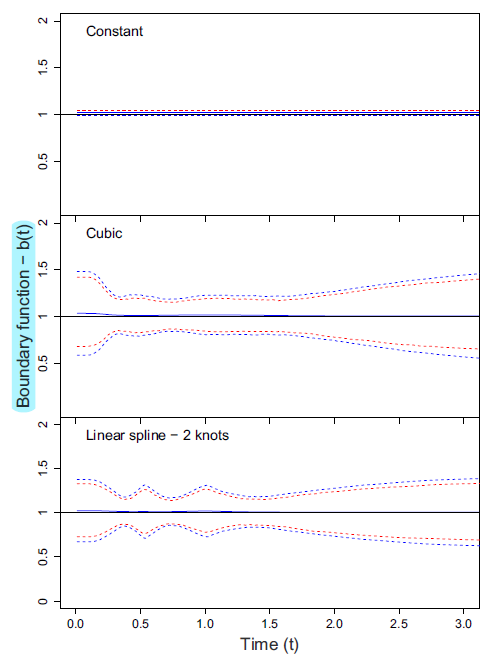
\includegraphics[angle=0, width=5cm]{graph.png}
            %\label{fig}
        \end{figure}
\end{frame}
%------------------------------------------------
\begin{frame}[noframenumbering]
    \label{Terms}
    \frametitle{Appendix - Terms}

    \begin{columns}[t] % The "c" option specifies centered vertical alignment while the "t" option is used for top vertical alignment
        \begin{column}{0.5\textwidth} % Right column width
            Some Estimators:
            \begin{itemize}
                \item Drift: $\hat{\delta}$
                \item Boundary: $\hat{b}(t)$
            \end{itemize}
        \end{column}
        \begin{column}{0.5\textwidth} % Left column width
            Some Variables:
            \begin{itemize}
                \item $\hat{V}$
                \item $\hat{m}_S$
                \item $\bar{m}$
                \item $m_J(\tau)$\newline\newline
            \end{itemize}
        \end{column}
    \end{columns}
    \hyperlink{Maths}{\beamerreturnbutton{Return to presentation}}
\end{frame}
%------------------------------------------------
\begin{frame}[noframenumbering, fragile]
\label{Code}
\frametitle{Appendix - Code Blocks}

\begin{minipage}{0.5\paperwidth}
\begin{lstlisting}[language=TeX]
\begin{itemize}
\item A \item B
\item C
\begin{itemize}
    \item C-1
\end{itemize}
\end{itemize}
\end{lstlisting}
\end{minipage}\hspace{1cm}
\begin{minipage}{0.3\paperwidth}
    \begin{itemize}
    \item A \item B
    \item C
    \begin{itemize}
        \item C-1
    \end{itemize}
    \end{itemize}
\end{minipage}\vspace{0cm}
\begin{minipage}{0.5\paperwidth}
\begin{lstlisting}[language=TeX]
\begin{enumerate}
\item A \item B
\item C
\end{enumerate}
\end{lstlisting}
\end{minipage}\hspace{1cm}
\begin{minipage}{0.5\paperwidth}
\begin{lstlisting}[language=TeX]
\begin{enumerate}
\item A \item B
\item C
\end{enumerate}
\end{lstlisting}
\end{minipage}

\hyperlink{Maths}{\beamerreturnbutton{Return to presentation}}
\end{frame}
%------------------------------------------------
\begin{frame}[noframenumbering]
\label{Theorems}
	\frametitle{Appendix - Theorems}
    \begin{enumerate}
        \item A single-line equation \newline
        
        \begin{equation*}
            J(\theta) = \mathbb{E}_{\pi_\theta}[G_t] = \sum_{s\in\mathcal{S}} d^\pi (s)V^\pi(s)=\sum_{s\in\mathcal{S}} d^\pi(s)\sum_{a\in\mathcal{A}}\pi_\theta(a|s)Q^\pi(s,a)
        \end{equation*}

        \item A multi-line equation with numbering \newline
        
        \begin{align}
            Q_\mathrm{target}&=r+\gamma Q^\pi(s^\prime, \pi_\theta(s^\prime)+\epsilon)\\
            \epsilon&\sim\mathrm{clip}(\mathcal{N}(0, \sigma), -c, c)\nonumber
        \end{align}
    \end{enumerate}

    \hyperlink{Maths}{\beamerreturnbutton{Return to presentation}}
\end{frame}

\end{document}
